%%%%%%
%
% $Autor: Wings $
% $Datum: 2020-01-18 11:15:45Z $
% $Pfad: WuSt/Skript/Produktspezifikation/powerpoint/ImageProcessing.tex $
% $Version: 4620 $
%
%%%%%%


\section{Optimierung der Trainingszeit}

% Auf der Website \url{https://www.kdnuggets.com/2020/03/tensorflow-optimizing-training-time-performance.html}findet sich ein TensorFlow 2.0 Tutorial zur Optimierung der Trainingszeit.

Werden die neuronalen Netze größer und komplexer, so erhöhen sich die Trainigszeiten. Daher ist es sinnvoll, sich um die Reduzierung der Trainigszeiten zu bemühen. Dazu stehen verschiedene Ansatzpunkte zur Verfügung:

\begin{enumerate}
    \item tf.data
    \item Mixed Precision Training
    \item Multi-\ac{gpu} Training Strategy
\end{enumerate}

Insgesamt kann die Trainingszeit um den Faktor 2 - 10 beschleunigt werden. \cite{KDnuggets.11.12.2020}

\subsection{Engpass identifizieren}

Bei Verwendung einer Grafikkarte der Firma NVIDIA ist die einfachste Lösung zur Überwachung der \ac{gpu}-Auslastung über die Zeit wahrscheinlich das Werkzeug \SHELL{nvtop}. Eine mögliche Ausgabe ist in Abbildung~\ref{Fignvtop} dargestellt. 

\begin{figure}[H]
    \begin{center}
        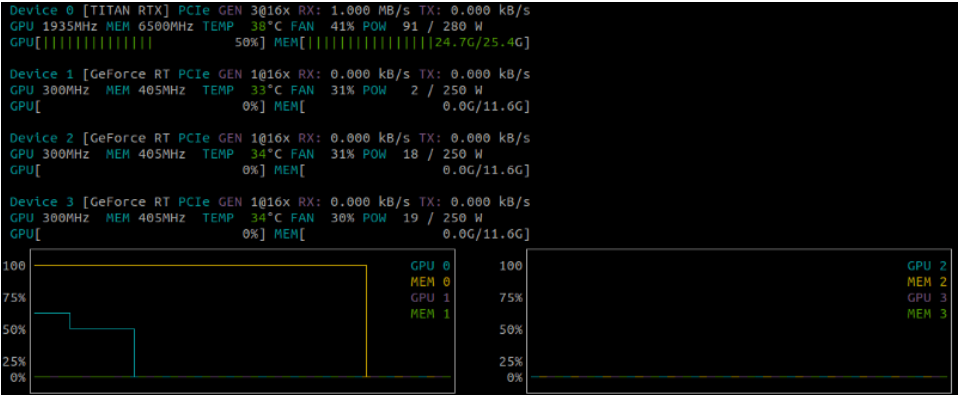
\includegraphics[width=0.9\textwidth]{TensorFlow/nvtop}
        \caption{Visualisierung von Engpässung mit \SHELL{nvtop} Quelle:\cite{KDnuggets.11.12.2020}} 
        \label{Fignvtop}
    \end{center}
\end{figure}

Zur Visualisierung der Auslastung mit TensorBoard muss 

\medskip

\PYTHON{profile\_batch=\{BATCH\_INDEX\_TO\_MONITOR\}}

\medskip

im TensorBoard als Callback-Funktion hinzugefügt werden. Dann wird ein vollständiger Bericht über die Operationen erstellt, die entweder von der \ac{cpu} oder der \ac{gpu} für den gegebenen Batch durchgeführt wurden. Dies kann dabei helfen, zu erkennen, ob der Prozessor an einem bestimmten Punkt aufgrund fehlender Daten blockiert ist.

\begin{figure}[H]
    \begin{center}
        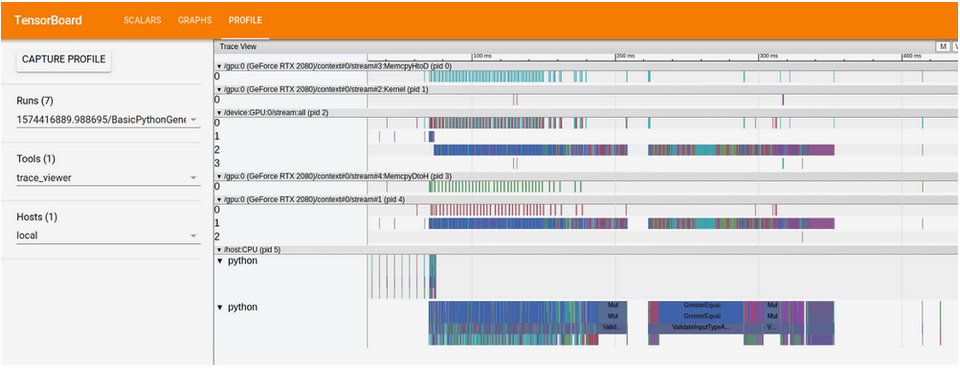
\includegraphics[width=0.9\textwidth]{TensorFlow/TensorBoardBottleneck}
        \caption{Visualisierung von Engpässung mit TensorBoard Quelle:\cite{KDnuggets.11.12.2020}} 
        \label{TensorBoardBottleneck}
    \end{center}
\end{figure}

\subsection{tf.data}

\Mynote{Hilft dies auch bei einer CPU?}

Um die \ac{gpu} durchgängig arbeiten zu lassen, muss der Engpass des Ladens der Daten  beseitigt werden. In Abbildung~\ref{TensorBoardBottleneckData} ist zu erkennen, dass die \ac{gpu} nicht arbeitet, während die \ac{cpu} mit dem Laden von Daten beschäftigt ist.

\begin{figure}[H]
    \begin{center}
        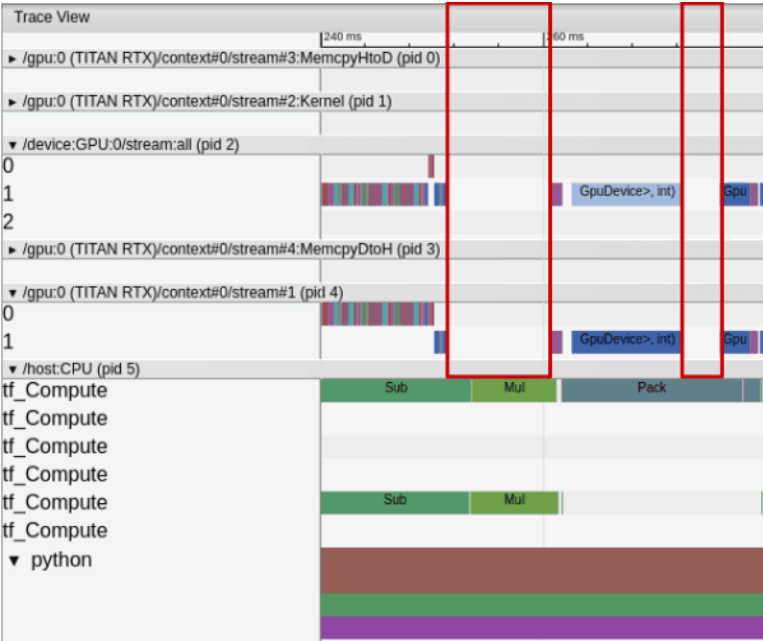
\includegraphics[width=0.9\textwidth]{TensorFlow/TensorBoardBottleneckData}
        \caption{Bottleneck Daten laden Quelle:\cite{KDnuggets.11.12.2020}} 
        \label{TensorBoardBottleneckData}
    \end{center}
\end{figure}

Als erstes sollte zur Beseitigung dieses Engpasses von Keras \PYTHON{sequences} zu \PYTHON{tf.data} gewechselt werden. Danach können weitere Optimierungen vorgenommen werden:

\begin{enumerate}
    \item Parallelisierung: Mit \PYTHON{num\_parallel\_calls\=tf.data.experimental.AUTOTUNE} werden die Aufrufe der Funktion  \PYTHON{.map()}  parallelisiert
    \item Cache: Der Cache kann verwendet werden , um geladene Bilder im Speicher zu halten. Dies kann durch das Zwischenspeichern von Datensätzen vor der Patch-Auswahl geschehen.
    \item Prefetching: Es werden Elementen abgerufen, bevor der vorherige Batch beendet wurde.
\end{enumerate}

Das nachfolgende Beispiel ist ein optimierter Code zur Datensatzerstellung mit scharfen und verschwommenen Bildern zu sehen:

\begin{code}
    \begin{lstlisting}[numbers=none]
        #dataset creation for optimizing training time
        #from https://www.kdnuggets.com/2020/03/tensorflow-optimizing-training-time-performance.html
        
        from pathlib import Path
        
        import tensorflow as tf
        
        def select_patch(sharp, blur, patch_size_x, patch_size_y):
        """
        Select a patch on both sharp and blur images at the same localization.
        Args:
        sharp (tf.Tensor): Tensor for the sharp image
        blur (tf.Tensor): Tensor for the blur image
        patch_size_x (int): Size of patch along x axis
        patch_size_y (int): Size of patch along y axis
        Returns:
        Tuple[tf.Tensor, tf.Tensor]: Tuple of tensors with shape (patch_size_x, patch_size_y, 3)
        """
        stack = tf.stack([sharp, blur], axis=0)
        patches = tf.image.random_crop(stack, size=[2, patch_size_x, patch_size_y, 3])
        return (patches[0], patches[1])
        
        
        class TensorflowDatasetLoader:
        def __init__(self, dataset_path, batch_size=4, patch_size=(256, 256), n_epochs=10, n_images=None):
        # List all images paths
        sharp_images_paths = [str(path) for path in Path(dataset_path).glob("*/sharp/*.png")]
        if n_images is not None:
        sharp_images_paths = sharp_images_paths[0:n_images]
        
        # Generate corresponding blurred images paths
        blur_images_paths = [path.replace("sharp", "blur") for path in sharp_images_paths]
        
        # Load sharp and blurred images
        sharp_dataset = tf.data.Dataset.from_tensor_slices(sharp_images_paths).map(
        lambda path: self.load_image(path, dtype),
        num_parallel_calls=tf.data.experimental.AUTOTUNE,
        )
        blur_dataset = tf.data.Dataset.from_tensor_slices(blur_images_paths).map(
        lambda path: self.load_image(path, dtype),
        num_parallel_calls=tf.data.experimental.AUTOTUNE,
        )
        
        dataset = tf.data.Dataset.zip((sharp_dataset, blur_dataset))
        dataset = dataset.cache()
        
        # Select the same patch on the sharp image and its corresponding blurred
        dataset = dataset.map(
        lambda sharp_image, blur_image: select_patch(
        sharp_image, blur_image, patch_size[0], patch_size[1]
        ),
        num_parallel_calls=tf.data.experimental.AUTOTUNE,
        )
        
        # Define dataset characteristics (batch_size, number_of_epochs, shuffling)
        dataset = dataset.batch(batch_size)
        dataset = dataset.shuffle(buffer_size=50)
        dataset = dataset.repeat()
        dataset = dataset.prefetch(buffer_size=tf.data.experimental.AUTOTUNE)
        
        self.dataset = dataset
        
        @staticmethod
        def load_image(image_path, dtype):
        image = tf.io.read_file(image_path)
        image = tf.image.decode_png(image, channels=3)
        image = tf.image.convert_image_dtype(image, dtype)
        image = (image - 0.5) * 2
        
        return image
    \end{lstlisting}
    
    \caption{Optimierter Code zur Datensatzerstellung mit scharfen und verschwommenen Bildern}
\end{code}


\subsection{Mixed Precision Training}

Standardmäßig werden alle Variablen als float32 gespeichert, also mit 32Bit. Mixed Precision Training beruht auf der Einsicht, dass diese hohe Präzision nicht immer benötigt wird, sodass an einigen Stellen auch 16 Bit genutzt werden können. Die Gewichte selber werden weiterhin als float32 Version gespeichert, Vorwärts- und Rückwärtspropagation nutzen aber die float16-Elemente. Die Genauigkeit wird so nicht verschlechtert, in einigen Fällen sogar erhöht.

Das Mixed Precision Training kann in TensorFlow Versionen ab 2.1.0 leicht implementiert werden. Es kann mit diesen beiden Zeilen vor der Modellinstanziierung aktiviert werden:

\medskip

\PYTHON{policy = tf.keras.mixed\_precision.experimental.Policy('mixed\_float16')}

\PYTHON{tf.keras.mixed\_precision.experimental.set\_policy(policy)}

\medskip

\subsection{Multi-GPU-Training}

%todo neu formulieren}

Der einfachste Weg, Multi-\ac{gpu}-Training durchzuführen, ist die Verwendung der \PYTHON{MirroredStrategy}. Sie instanziiert das Modell auf jeder \ac{gpu}. Bei jedem Schritt werden verschiedene Batches an die \ac{gpu}s gesendet, die den Backward Pass \Mynote{Was ist Backward Pass?} ausführen. Dann werden die Gradienten aggregiert, um eine Aktualisierung der Gewichte durchzuführen, und die aktualisierten Werte werden  an jedes instanziierte Modell propagiert.

Die Verteilungsstrategie ist mit TensorFlow 2.0 wieder recht einfach. Es ist nur daran zu denken, dass die übliche Batchgröße mit der Anzahl der verfügbaren \ac{gpu}s zu multiplizieren:

\medskip
\PYTHON{\# Define multi-gpu strategy }

\PYTHON{mirrored\_strategy = tf.distribute.MirroredStrategy()}

\PYTHON{\# Update batch size value}

\PYTHON{batch\_size *= mirrored\_strategy.num\_replicas\_in\_sync}

\PYTHON{\# Create strategy scope to perform training}

\PYTHON{with mirrored\_strategy.scope():}

\PYTHON{\qquad  model = [...]}

\PYTHON{\qquad  model.fit(...)}


\section{Optimierung Multithreading}


Das Multithreading von Tensorflow kann zur Optimierung genutzt werden.

\Mynote{Neu formulieren}

\begin{itemize}
    \item \PYTHON{tf.config.threading}:
    \begin{itemize}
        \item \PYTHON{set\_intra\_op\_parallelism\_threads}: Legt die Anzahl der Threads fest, die innerhalb einer einzelnen Operation für Parallelität verwendet werden.
        \item \PYTHON{set\_inter\_op\_parallelism\_threads}: Legt die Anzahl der Threads fest, die für die Parallelität zwischen unabhängigen Vorgängen verwendet werden.
    \end{itemize}
    \item \FILE{OpenMP runtime} (aktiviert via \SHELL{os.environ[\ldots]}):
    \begin{itemize}
        \item \PYTHON{OMP\_NUM\_THREADS}: Anzahl der für OpenMP verfügbaren Threads.
        \item \PYTHON{KMP\_BLOCKTIME}: Die Zeit eines Spinlocks, gemessen in Millisekunden
        \item \PYTHON{KMP\_AFFINITY}: Definieren Sie die Zuordnung von Threads zu den Hardware-Ressourcen.
    \end{itemize}
\end{itemize}




Der Wert \PYTHON{OMP\_NUM\_THREADS} wird auf die Anzahl der verfügbaren Kernen und der Parameter \PYTHON{KMP\_BLOCKTIME} wird auf einen kleineren Wert als das größere Netz gesetzt.

\bigskip

Festlegung der Affinität:

\PYTHON{os.environ["KMP\_AFFINITY"]="granularity=fine,compact,1,0,verbose"}

\bigskip

\GRAPHICSC{1.0}{1.0}{TensorFlow/Knobs}

